\documentclass{beamer}
\usepackage{phdstyle}

\title{Effect of spin motion perturbation on the EDM statistic}
\author{Alexander Aksentev}
\date{\today}

\begin{document}
\begin{frame}
  \titlepage
\end{frame}
\begin{frame}
  \frametitle{Problem statement}
  \begin{columns}
    \begin{column}{.6\textwidth}
      \begin{itemize}
      \item The spin precession axis (SPA) of a particle involved in betatron motion moves about the invariant spin axis defined on the CO: $\vec\W = \vec\W_0(\Theta) + \vec\w(\Theta, \Delta\vec r)$.
      \item Simultaneously, it was claimed that: for two beams, $\gamma_{eff}^1(\frac{\Delta L}{L}, \frac{\Delta p}{p}) = \gamma_{eff}^2(\frac{\Delta L}{L}, \frac{\Delta p}{p}) \rightarrow (\W_x^1, \W_y^1, \W_z^1) = (\W_x^2, \W_y^2, \W_z^2) $, \textbf{regardless} of the particulars of their orbital motion.
      \end{itemize}
    \end{column}
    \begin{column}{.4\textwidth}
  \begin{center}
    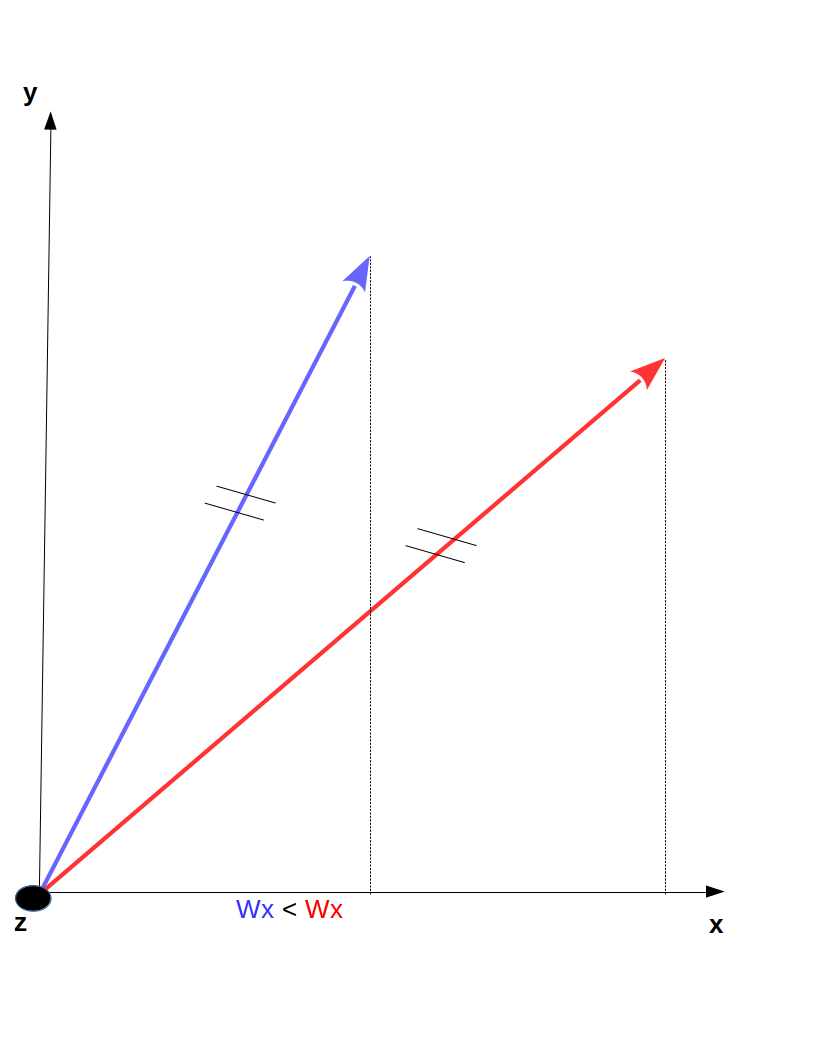
\includegraphics[height=.62\paperheight]{img/spin_axis_motion/presentation/nbar_arrows}
  \end{center}
  \end{column}
  \end{columns}
  The last statement makes sense so long as by ``frequency'' we mean $|\vec\W|$. Couldn't see how $\gamma_{eff}$ alone can guarantee the equality of the $\bar n$ orientations. Must be an implicit assumption.
\end{frame}

\begin{frame}
  \frametitle{Single particle $\nu_s$, $\bar n$, and $\W_x$}
  \textbf{Implicit assumption} (sic!): All spin vectors in the beam precess about the same $\bar n_{CO}$. (More carefuly: $\bar n_i - \bar n_{CO} \ll 1$.)\\
  \textbf{Below}: 270 MeV (FS@270.0092 MeV), FS lattice w/E+B elements tilted about the optic axis by $\theta\sim N(8\cdot10^{-2}, 10^{-2})$ rad. Observe a significant $\sigma[\W_x]$.\\
  \textbf{Hypothesis}: averaging out in the polarization vector.
  \vspace*{-.5cm}
  \begin{columns}
    \begin{column}{.5\textwidth}
      \begin{center}
        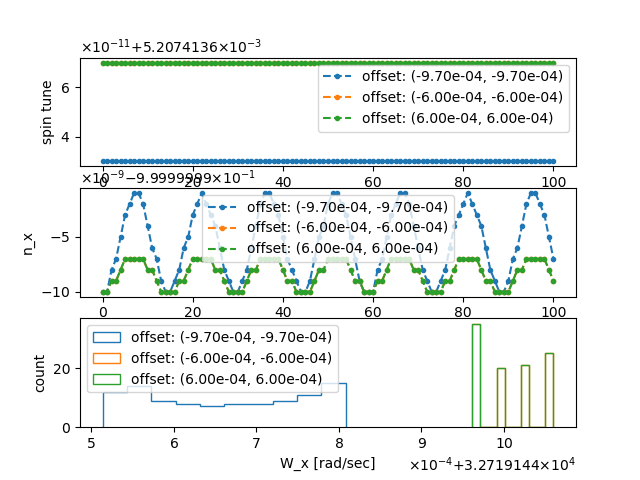
\includegraphics[height=.5\paperheight]{img/spin_axis_motion/presentation/spin_tune_three}
      \end{center}
    \end{column}
    \begin{column}{.5\textwidth}
      \begin{center}
        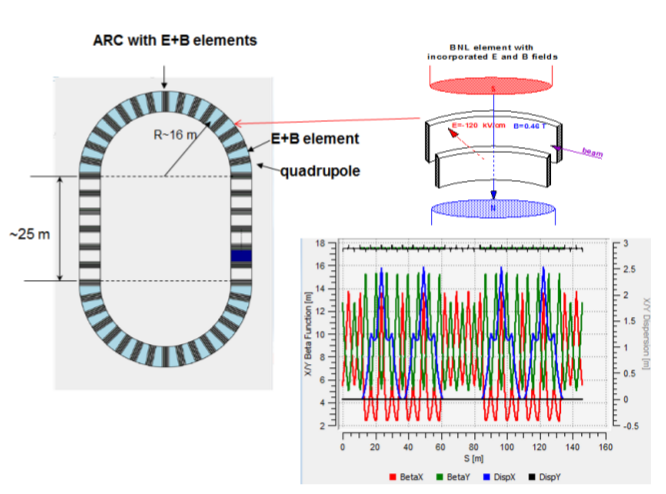
\includegraphics[height=.5\paperheight]{img/spin_axis_motion/presentation/lattice}
      \end{center}
    \end{column}
  \end{columns}
\end{frame}
\begin{frame}
  \frametitle{Simulation: Uniform beam}
  \begin{itemize}
    \item Same lattice; beam represented by 4,000 rays; $x_0,~y_0\in [-1mm, +1mm]$, $d_0:=\Delta K/K_{ref} \in [-10^{-4}, +10^{-4}]$.
    \item $\vec P = \frac{\sum_{i\in E} \vec s_i}{||\sum_{i\in E} \vec s_i||}.$
    \item Fit $P_y$ by model $g(t) = \sin(2\pi f\cdot t)$.
    \item Residuals exhibit a systematic pattern (model error); also $\hat f_{P_y} < \hat f_{s_y}^{CO}$.
    \item However, $\hat f_{P_y}^{CW} - \hat f_{P_y}^{CCW}$ is below statistical precision.
    %% \item Also, moving frame estimates don't exhibit a trend.
    \item But what if the CW \& CCW beams are \textbf{not} identical?
  \end{itemize}
  \vspace*{-.3cm}
  \begin{center}
    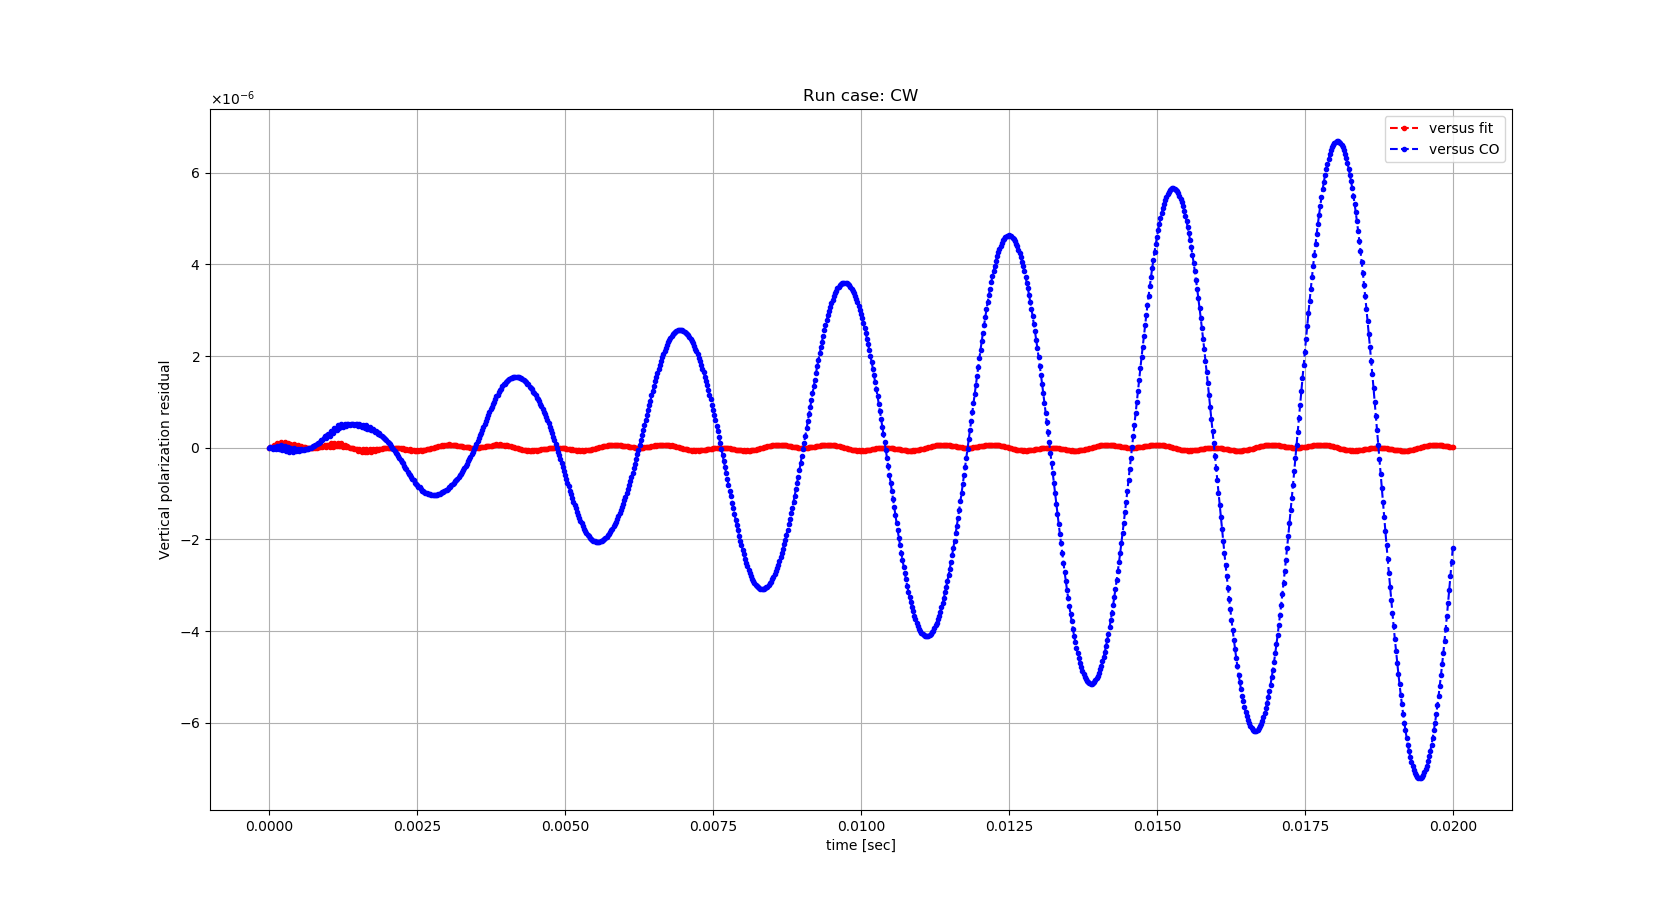
\includegraphics[height=.5\paperheight]{img/spin_axis_motion/CW_polarization_residual_full}
  \end{center}
\end{frame}
\begin{frame}
  \begin{center}
    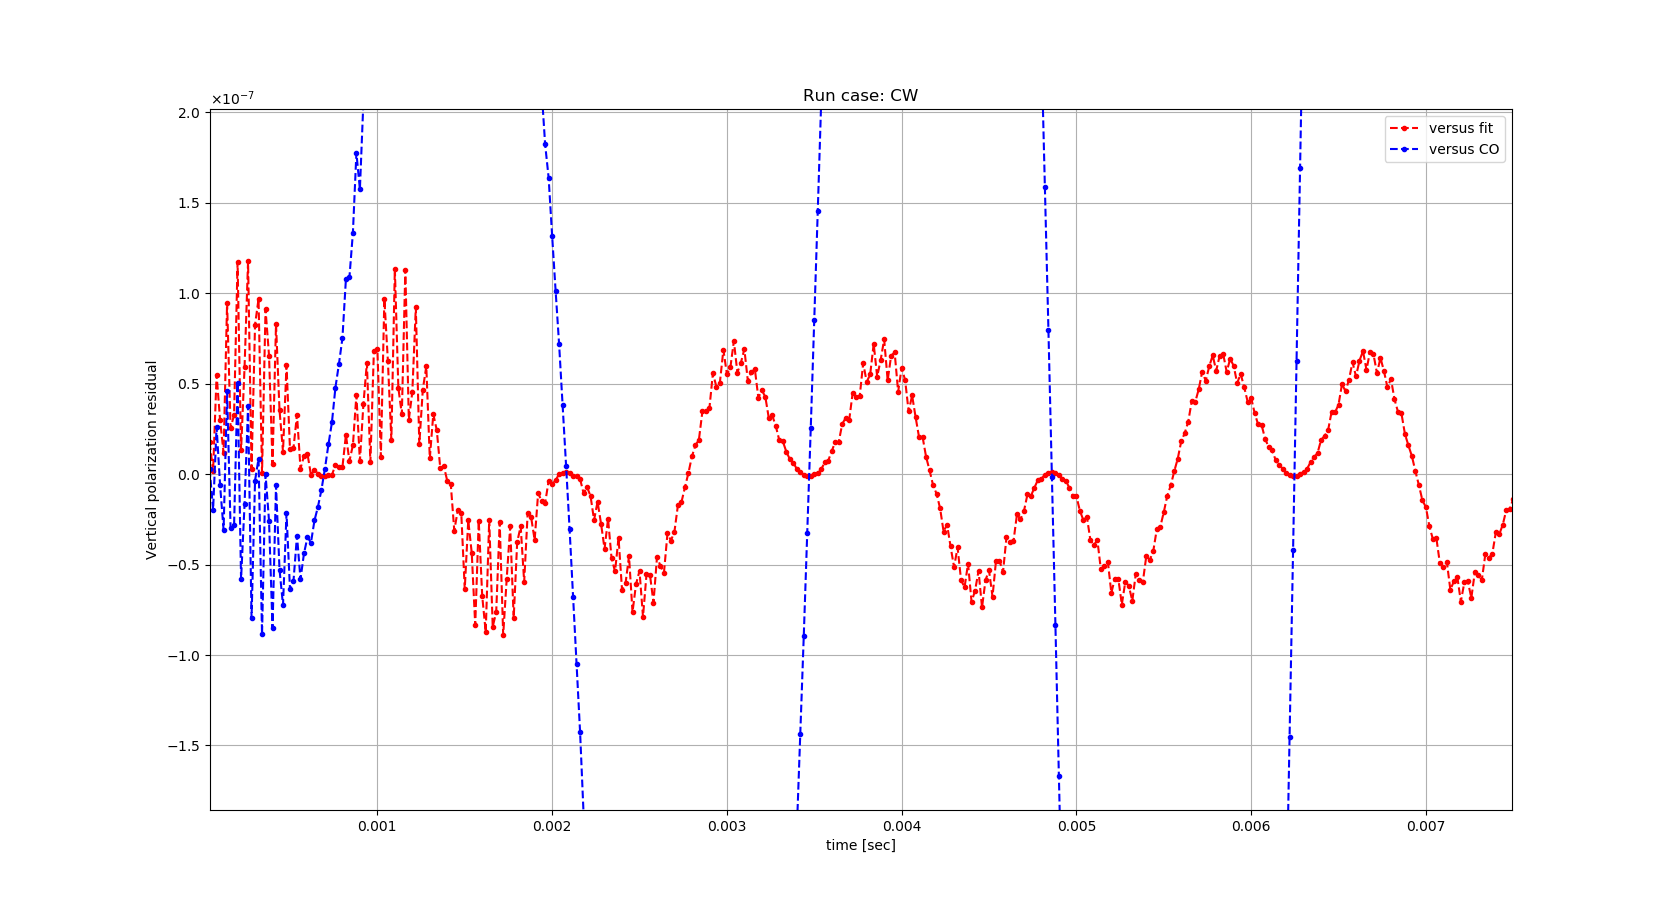
\includegraphics[height=.5\paperheight]{img/spin_axis_motion/CW_polarization_residual_cut}
  \end{center}
  \begin{center}
    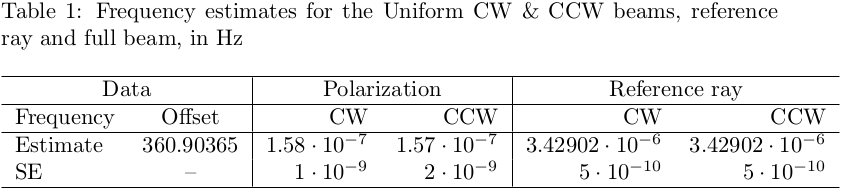
\includegraphics[height=.25\paperheight]{img/spin_axis_motion/presentation/uni_beam_table}
  \end{center}
\end{frame}

\begin{frame}
  \frametitle{Simulation: Gaussian beams}
  \vspace*{-.8cm}
  \begin{columns}
    \begin{column}{.5\textwidth}
      \begin{center}
        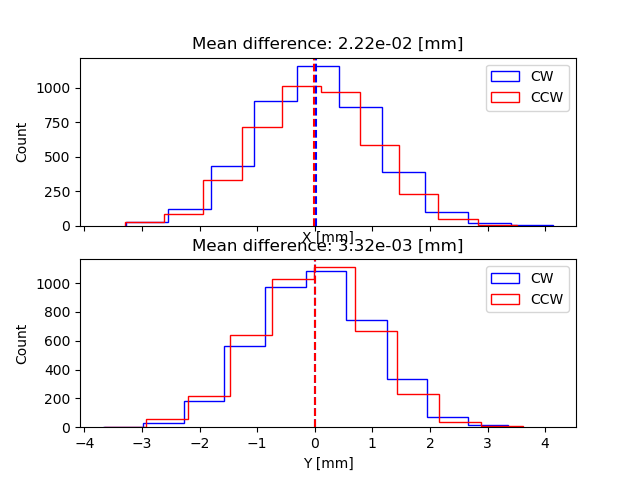
\includegraphics[height=.5\paperheight]{img/spin_axis_motion/gaussian_beam_histograms_XY}
      \end{center}
    \end{column}
    \begin{column}{.5\textwidth}
      \begin{center}
        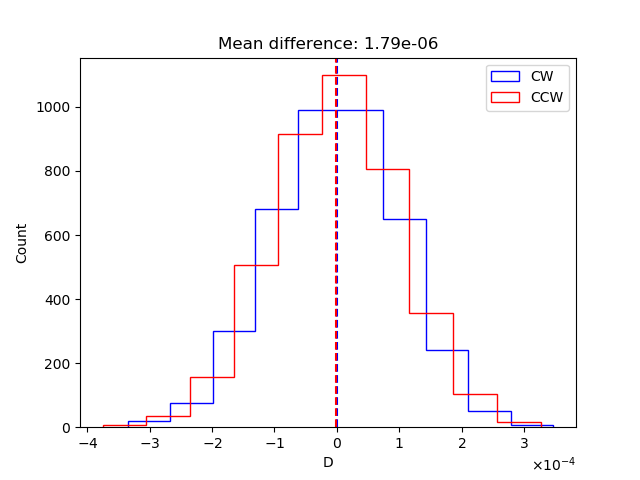
\includegraphics[height=.5\paperheight]{img/spin_axis_motion/gaussian_beam_histograms_D}
      \end{center}
    \end{column}
  \end{columns}
  \vspace*{-.2cm}
  \begin{center}
    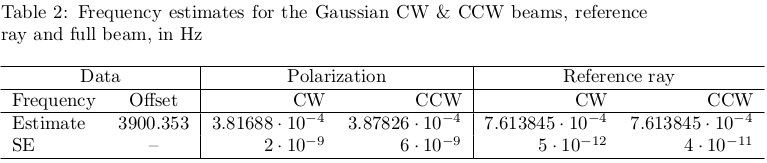
\includegraphics[height=.25\paperheight]{img/spin_axis_motion/presentation/gauss_beam_table}
  \end{center}
  \vspace*{-.3cm}
    Error: $\varepsilon := \hat f^{CW} - \hat f^{CCW} = 6\cdot 10^{-6}~\text{(model)} \pm 6\cdot 10^{-9}~\text{(fit)}$ Hz.
\end{frame}
\begin{frame}
  \frametitle{Multiple runs}
  \textbf{Hypothesis}: the systematic error component likely depends on the beam centroid difference. Define the centroid by $\vec c = (\avg{x_0}, \avg{y_0}, \avg{d_0})$. Then do linear regression of $\hat f^{CW} - \hat f^{CCW}$ on $\vec c^{CW} - \vec c^{CCW}$.
  \begin{center}
    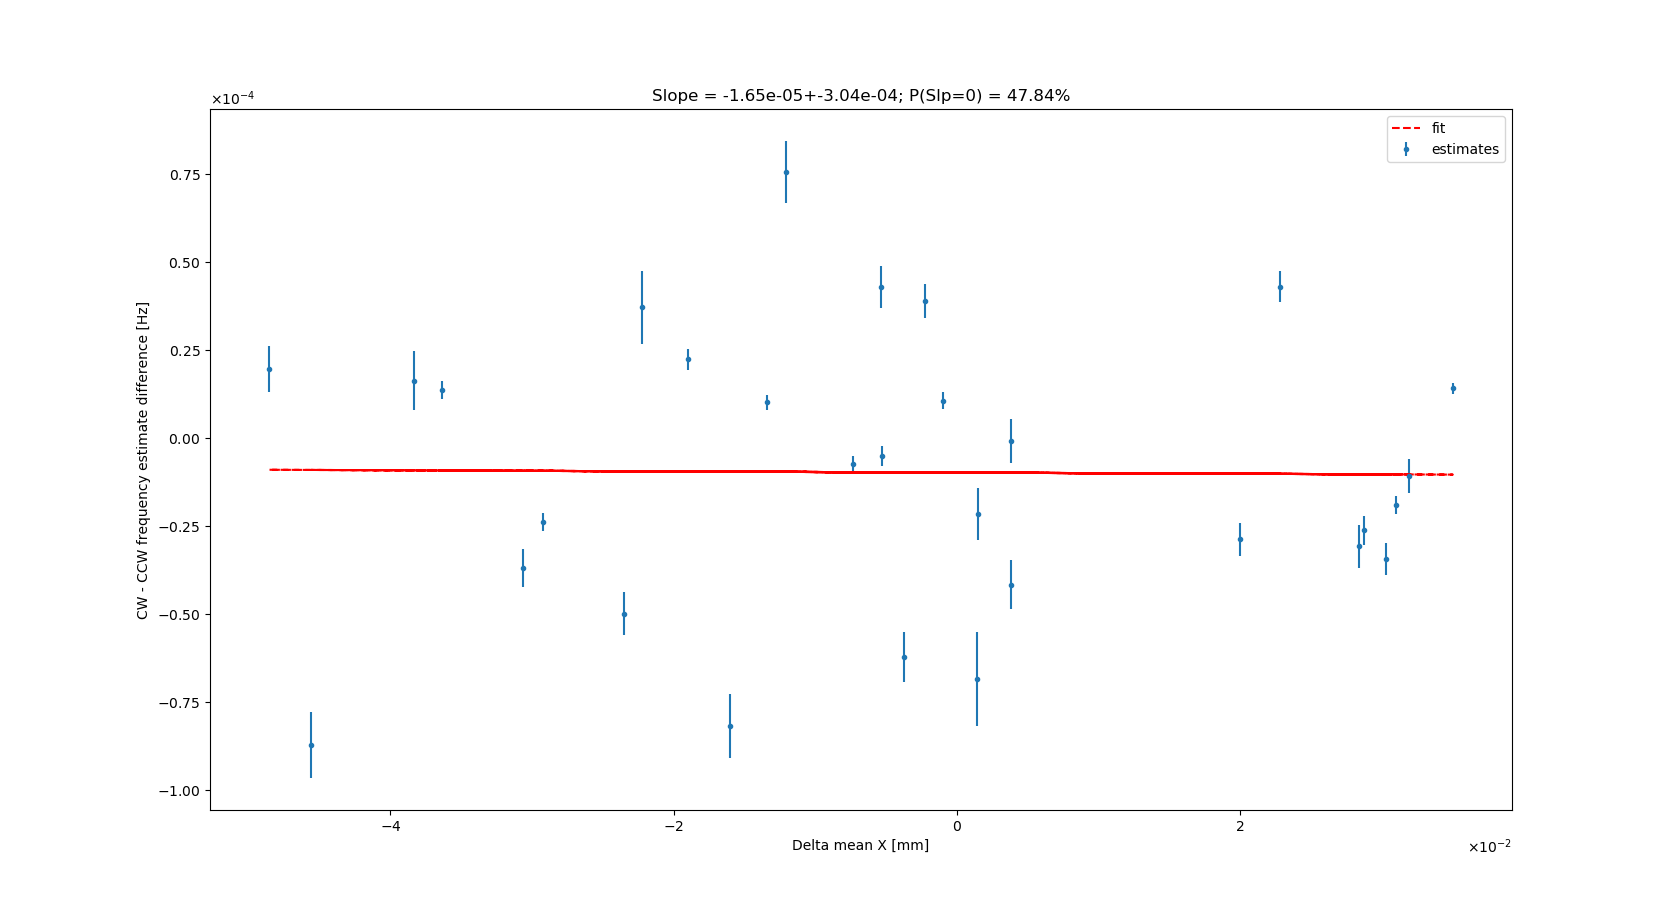
\includegraphics[height=.5\paperheight]{img/spin_axis_motion/freq_estimates_vs_centroid_diff_X}
  \end{center}
\end{frame}
\begin{frame}
  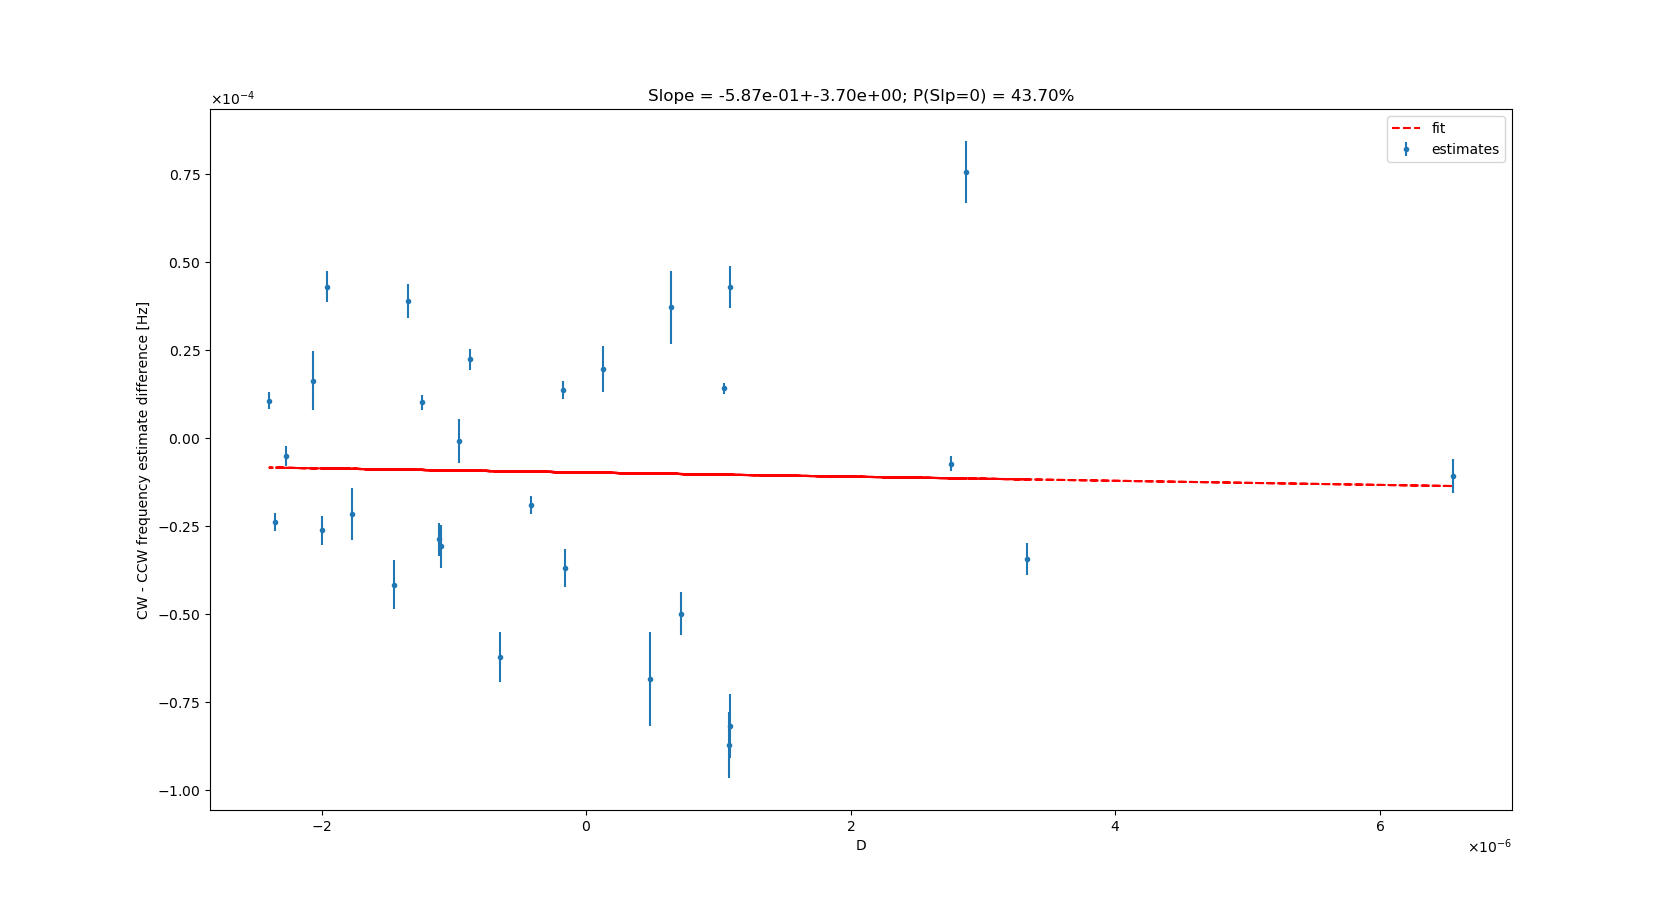
\includegraphics[height=.5\paperheight]{img/spin_axis_motion/freq_estimates_vs_centroid_diff_D}\\
  \vspace*{-.2cm}
  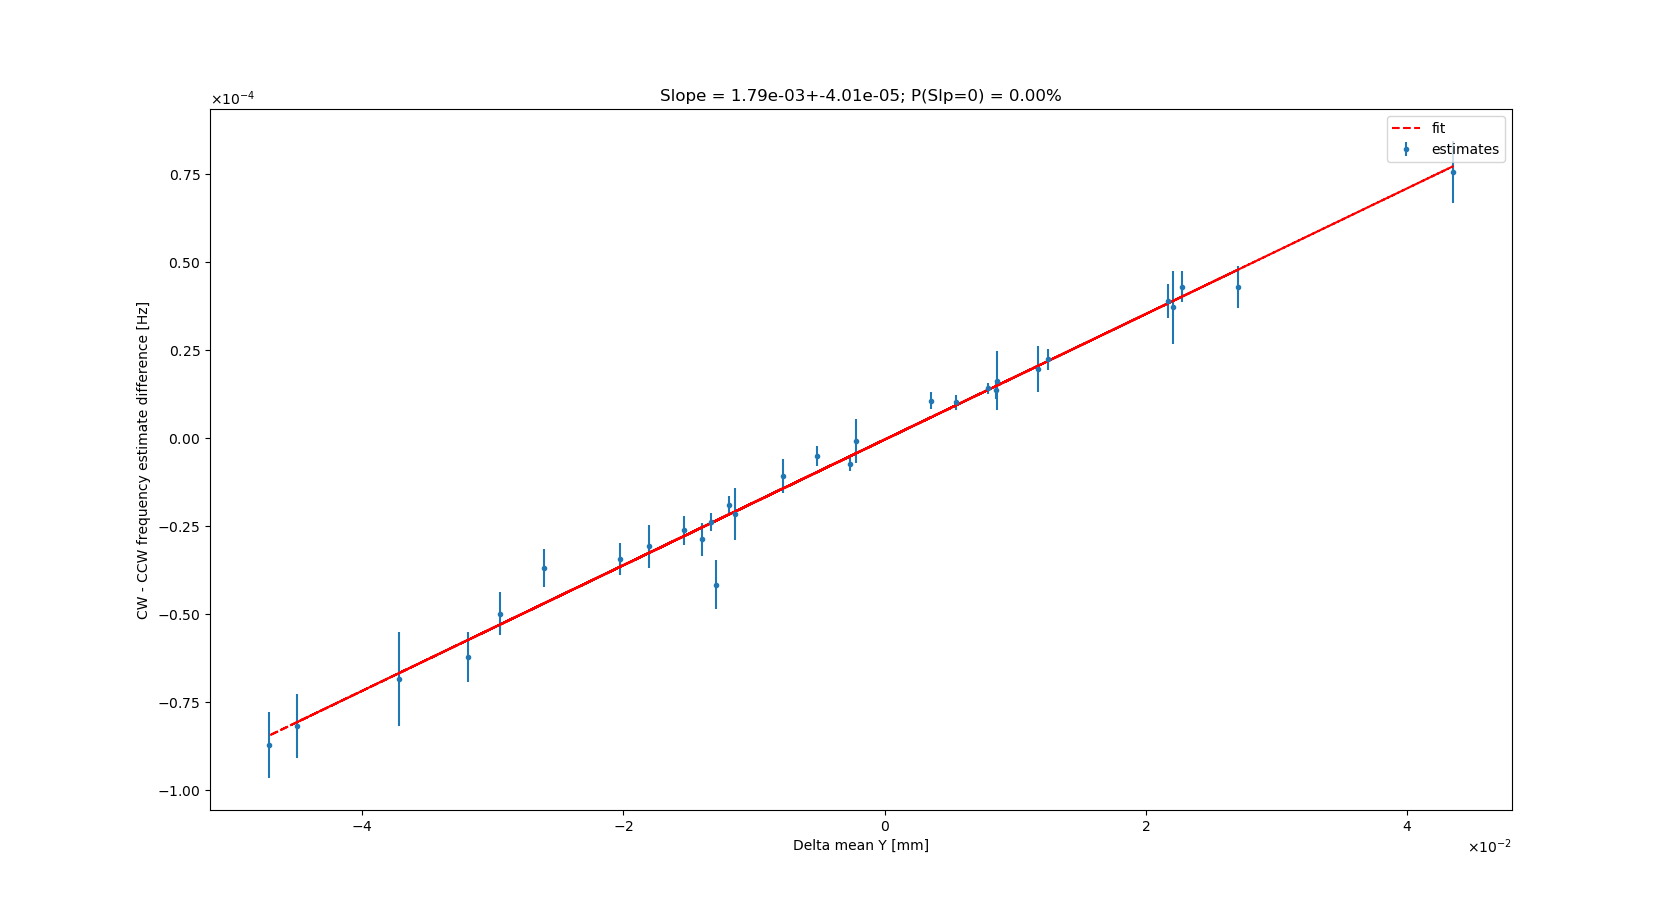
\includegraphics[height=.5\paperheight]{img/spin_axis_motion/freq_estimates_vs_centroid_diff_Y}
\end{frame}
\begin{frame}
  \frametitle{Effect size dependence on the beam size}
  \begin{itemize}
  \item $\varepsilon = a_0 + a_1\Delta \vec c_y$;
  \item all beams in the simulation had the same CO; $\vec c_y$ deviated from 0 only b/c of a finite sample size;
  \item $\sigma_{\avg{y}}\equiv \sigma_{4k} = \sigma/\sqrt{n}$, hence if $n = 4\cdot 10^3 \rightarrow n=4\cdot 10^9$, then $\sigma_{4b} = \sigma_{4k}\cdot 10^{-3}$;
  \item then the model part of $\varepsilon$ would also drop 3 orders of magnitude, and would be comparable with fit error.
  \end{itemize}
\end{frame}
\begin{frame}\frametitle{Extra}
  \begin{center}
    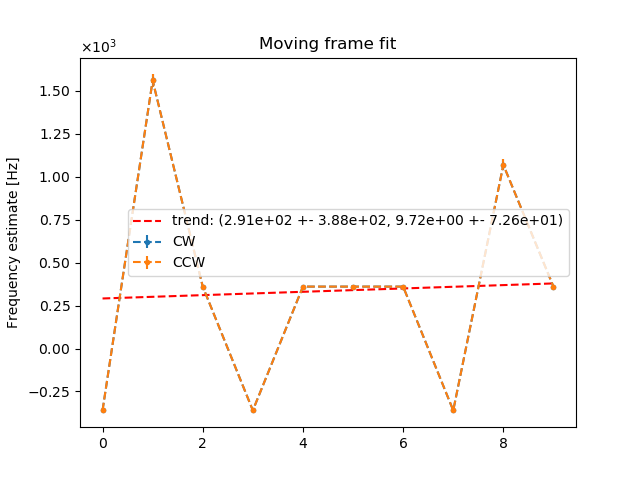
\includegraphics[height=.7\paperheight]{img/spin_axis_motion/moving_frame_freqs}
    %% \caption{Moving frame fit estimates.}
  \end{center}
\end{frame}
\end{document}

